\documentclass{beamer}
\setbeamertemplate{caption}[numbered]
\usetheme[numbers, totalnumbers, compress, nologo]{Statmod}

\title[Синолитические сети в класс. мозговой активности]{Синолитические сети в классификации мозговой активности}

\author[Власенко Д.В.]{Власенко Даниил Владимирович, гр.19.Б04-мм}

\institute[Санкт-Петербургский Государственный Университет]{%
	\small
	Научный руководитель: к.ф.-м.н. Шпилёв П.В.\\ \vspace{0.5cm}
	Санкт-Петербургский государственный университет\\
	Прикладная математика и информатика\\
	Вычислительная стохастика и статистические модели\\
	\vspace{1.25cm}
	Отчет по научно-исследовательской работе}

\date[Зачет]{Санкт-Петербург, 2023}

\makeatletter
\newcommand*{\rom}[1]{\expandafter\@slowromancap\romannumeral #1@}
\makeatother

\usepackage{amsmath,amssymb,amsthm,amscd,amsfonts, mathtools}
\usepackage[utf8]{inputenc}
\usepackage[english, russian]{babel}
\usepackage{wrapfig}
\usepackage{multirow}

\newtheorem{defenition}{Определение}
\newtheorem*{fMRI*}{Функциональная магнитно-резонансная томография}
\newtheorem*{classification*}{Задача классификации}
\newtheorem*{purpose*}{Цель работы}
\newtheorem*{prob_task*}{Вероятностная постановка задачи классификации}
\newtheorem*{algo_task*}{Алгоритмическая постановка задачи классификации}
\newtheorem*{prob_def*}{Вероятностное определение $w_{ij}$}
\newtheorem*{algo_def*}{Алгоритмическое определение $w_{ij}$}

\begin{document}
	\title[Синолитические сети в класс. мозговой активности]{Синолитические сети в классификации мозговой активности}
	
	\author[Власенко Д.В.]{Власенко Даниил Владимирович, гр.19.Б04-мм}
	
	\institute[Санкт-Петербургский Государственный Университет]{%
		\small
		Научный руководитель: к.ф.-м.н. Шпилёв П.В.\\ \vspace{0.5cm}
		Санкт-Петербургский государственный университет\\
		Прикладная математика и информатика\\
		Вычислительная стохастика и статистические модели\\
		\vspace{1.25cm}
		Отчет по научно-исследовательской работе}
	
	\date[Зачет]{Санкт-Петербург, 2023}
	
		
	\begin{frame}
		\titlepage
	\end{frame}

	\section{Введение}
		\subsection{фМРТ, векторизация данных}
			\begin{frame}	
				\begin{fMRI*}
					 Разновидность магнитно-резонансной томографии, которая проводится с целью измерения изменений в токе крови, вызванных нейронной активностью головного мозга.
				\end{fMRI*}	 
				\vspace{0.5cm}
				
				\begin{figure}
					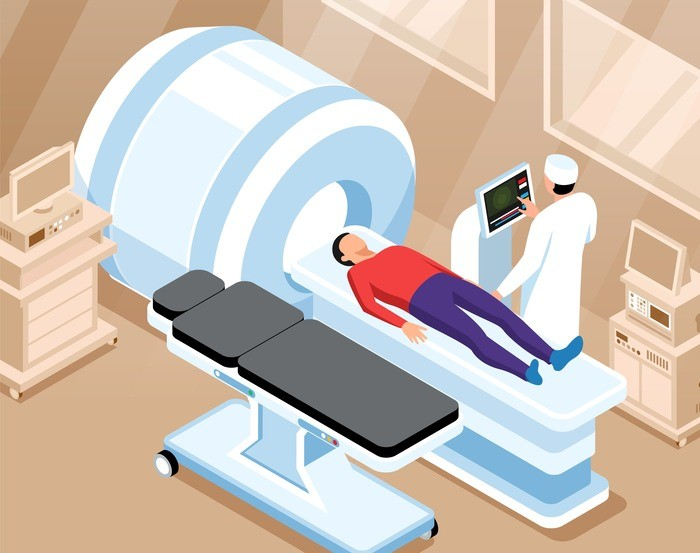
\includegraphics[width=5cm]{../images/fmri_1.jpeg}
					\caption{фМРТ сканер.} 
					\label{fg:1}
				\end{figure}	
			\end{frame}
	
		\subsection{Классификация, представление мозга как сети}
			\begin{frame}
				\begin{classification*}
					Пусть $\Omega$ --- множество объектов, $\Sigma$ --- множество классов. Существует неизвестная функция $f: \Omega \rightarrow \Sigma$, значения которой известны только на объектах выборки $(\widetilde{\Omega}, \widetilde{\Sigma}) =  \{(\omega_{n}, \sigma_{n})\}_n$. 
					\vspace{0.35cm}
					
					Требуется построить алгоритм $\widehat{f}: \Omega \rightarrow \Sigma$, способный классифицировать произвольный объект $\omega \in \Omega$, то есть правильно сопоставить ему соответствующий класс $\sigma \in \Sigma$.
				\end{classification*}
					
				\begin{figure}
					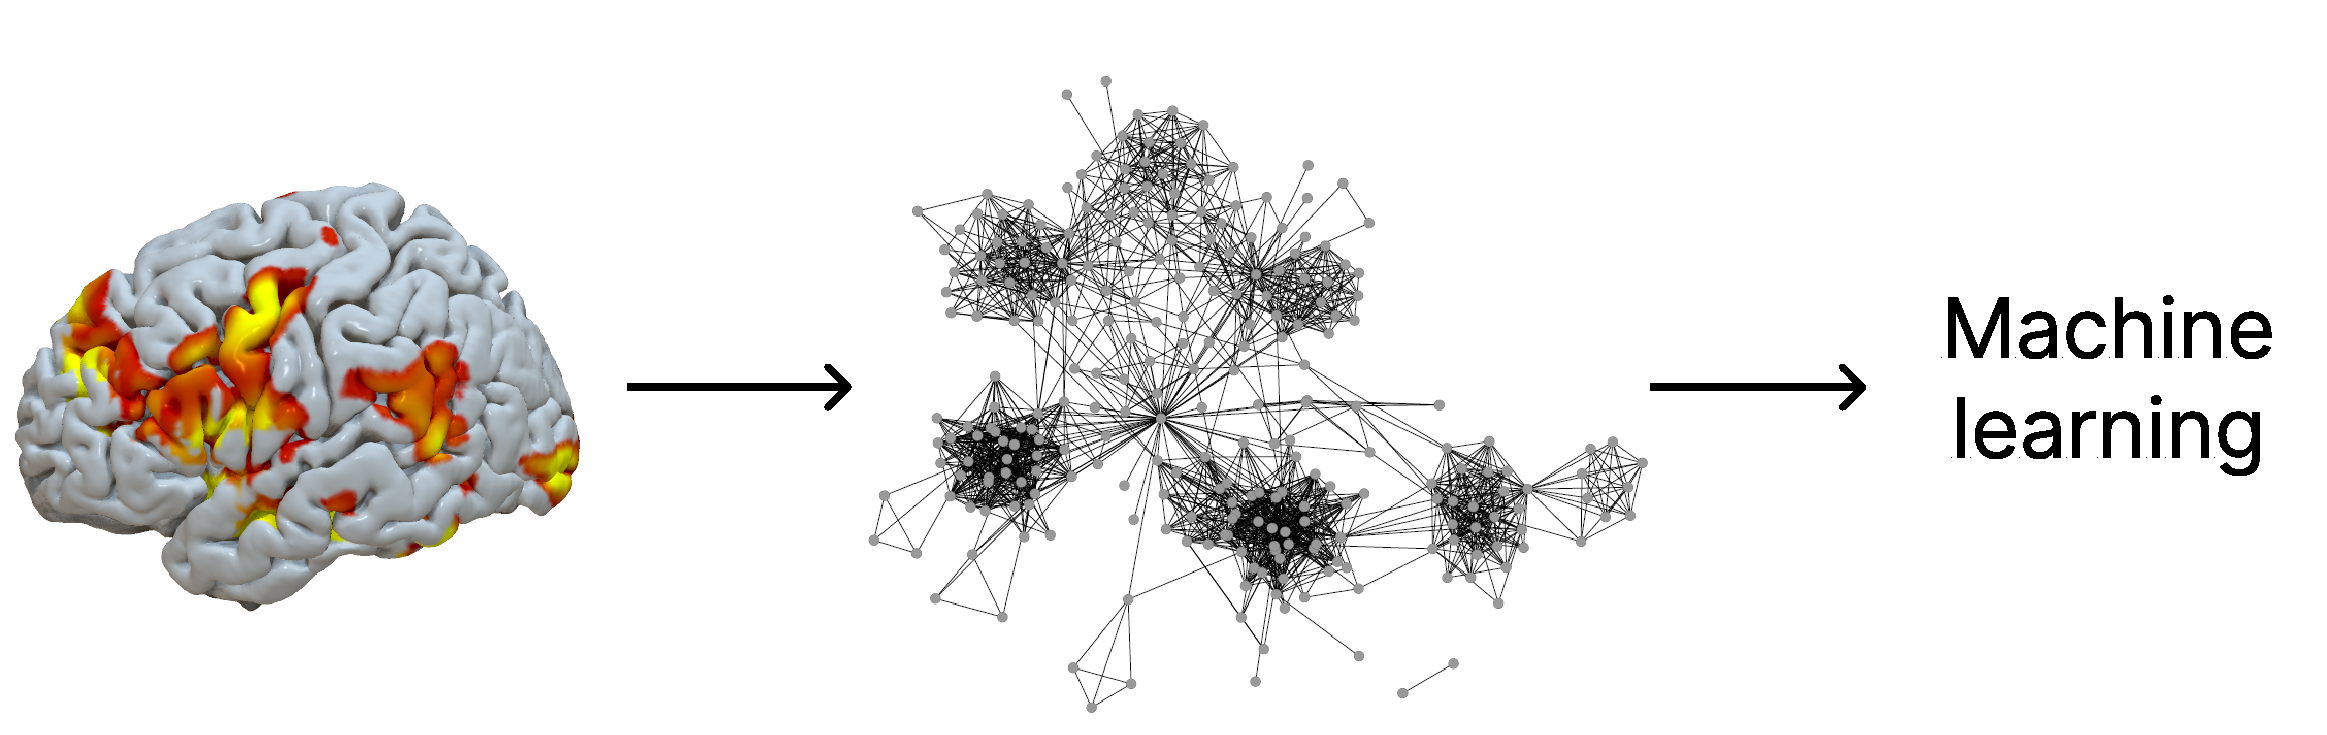
\includegraphics[width=10cm]{../images/fmri_graph_ml_1.pdf}
					\caption{Классификация на основе характеристик графов, содержащих информацию о работе мозга.} 
					\label{fg:3}
				\end{figure}						
			\end{frame}
		
		\subsection{Цель работы}
			\begin{frame}		
				\begin{purpose*}
					Реализация и тестирование метода классификации режимов мозговой активности на основе фМРТ данных, в основе которого будут лежать синолитические сети (Zaikin Alexey 2022).
				\end{purpose*}
			\end{frame}
		
	\section{Модель}
		\subsection{Построение графа на основе фМРТ}
			\begin{frame}		
				$\Omega$ --- множество фМРТ, а $\Sigma = \{$\rom{1}, \rom{2}$\}$ --- множество режимом мозговой активности. $(\widetilde{\Omega}, \widetilde{\Sigma}) =  \{(\omega_{n}, \sigma_{n})\}_n$ --- конечная выборка из $(\Omega, \Sigma)$.		
				
				\begin{enumerate}
					\setcounter{enumi}{0}
					\item $\omega \in \Omega$ конвертируется массив~$a$. $a_{xyzt}$ --- значение вокселя с индексами $x$, $y$, $z$ в момент времени $t$, а $a_{xyz}$ --- все значения вокселя с индексами $x$, $y$, $z$.
				\end{enumerate}
				
				На основе $a$ будет строится граф $g = (V = \{v_i\}_i, E = \{e_{ij}\}_{ij},$\\$ R = \{r_i\}_i, W = \{w_{ij}\}_{ij})$.
				
				\begin{enumerate}
					\setcounter{enumi}{1}
					\item С помощью статистики $T$ вычисляется $a^{T} = T(a)$, т.е для $\forall x, y, z$ $a^{T}_{xyz} = T(a_{xyz})$. Значения массива $a^{T}$ будут использоваться в качестве значений вершин $R$.					
				\end{enumerate}														
			\end{frame}
		
			\begin{frame}		
				\begin{prob_def*}
					\begin{equation*}
						w_{ij} = P(y_k = \rom{2} | r_i, r_j) - P(y = \rom{1} | r_i, r_j)
					\end{equation*}
				\end{prob_def*}				
				
				\begin{enumerate}
					\setcounter{enumi}{2}
					\item С помощью классификаторов $Cl_{ij}: \{y |(r_i, r_j), \{(r_i^n, r_j^n)\}_n,$\\$ \{y_n\}_n\} \rightarrow [0, 1]$, обученных на выборке $(\widetilde{\Omega}, \widetilde{\Sigma})$, вычисляется $W$.
					\item Строиться граф-сетка $g$, т.е. граф, в котором каждый внутренний воксель связан с 26 соседними вокселями.
				\end{enumerate}	
					
			\end{frame}

			


\end{document}